\let\negmedspace\undefined
\let\negthickspace\undefined
\documentclass[journal,12pt,twocolumn]{IEEEtran}
\usepackage{cite}
\usepackage{amsmath,amssymb,amsfonts,amsthm}
\usepackage{algorithmic}
\usepackage{graphicx}
\usepackage{textcomp}
\usepackage{xcolor}
\usepackage{txfonts}
\usepackage{listings}
\usepackage{enumitem}
\usepackage{mathtools}
\usepackage{gensymb}
\usepackage{comment}
\usepackage[breaklinks=true]{hyperref}
\usepackage{tkz-euclide} 
\usepackage{listings}
\usepackage{gvv}                                        
\def\inputGnumericTable{}                                 
\usepackage[latin1]{inputenc}                                
\usepackage{color}                                            
\usepackage{array}                                            
\usepackage{longtable}                                       
\usepackage{calc}                                             
\usepackage{multirow}                                         
\usepackage{hhline}                                           
\usepackage{ifthen}                                           
\usepackage{lscape}
\usepackage{caption}
\newtheorem{theorem}{Theorem}[section]
\newtheorem{problem}{Problem}
\newtheorem{proposition}{Proposition}[section]
\newtheorem{lemma}{Lemma}[section]
\newtheorem{corollary}[theorem]{Corollary}
\newtheorem{example}{Example}[section]
\newtheorem{definition}[problem]{Definition}
\newcommand{\BEQA}{\begin{eqnarray}}
\newcommand{\EEQA}{\end{eqnarray}}
\newcommand{\define}{\stackrel{\triangle}{=}}
\theoremstyle{remark}
\newtheorem{rem}{Remark}
\begin{document}

\bibliographystyle{IEEEtran}
\vspace{3cm}

\title{10.5.2.14}
\author{EE23BTECH11003 - pranav}
\maketitle
\newpage

\bigskip


\textbf{Question}:
no of multiples of 4 between 10 and 250
\\let $4n_{1}$ and $4n_{2}$ be the first and last multiples of 4 between 10 and 250 then\\ 

 $4n_{1}>10$  $\&$ $4n_{2}<250$  \\
 $\implies$ $n_{1}>10/4$ $\&$ $n_{2}<250/4$\\
$ \therefore$ $n_{1}$ $\&$ $n_{2}$ $\in$ $\mathbb{N}$\\
 $\implies$ $n_{1}=3$ $n_{2}=62$ \\
 $\therefore$ no of multiples of 4 between 10 and 250 are $62-3+1=60$ \\
considering the series to start from $n=0$ the general term
\begin{align}
S(n)=S(0)+n\cdot d\\
S(n)=12+4\cdot n
\end{align}
\begin{table}[h]
    \centering
    \input{tables/Table.Tex}
    \caption{Variables Used}
    \label{tab	: 10.5.2.14}
\end{table}
\begin{figure}[h!]
    \centering
    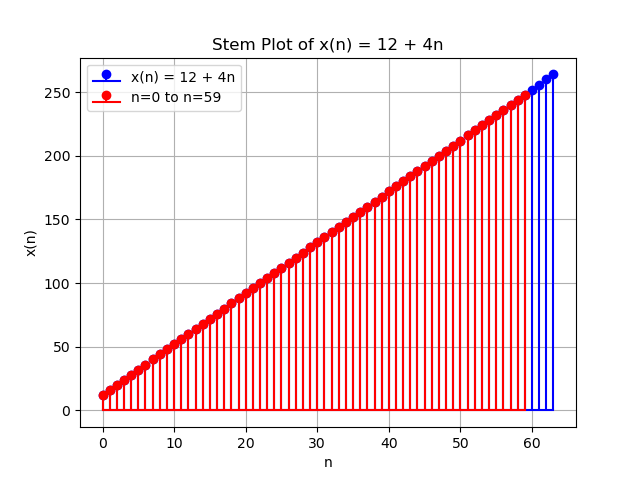
\includegraphics[width=1.1\linewidth]{figs/graph1.png}
    \caption{general term of the AP}
    \label{fig:enter-label}
\end{figure}

\end{document}
